\subsection{Задание 1. Реализация библиотеки поиска максимального элемента}

В рамках задания была разработана библиотека, реализующая функцию поиска максимального элемента в массиве. Требовалось реализовать функцию двумя способами: \textbf{итеративным} и \textbf{рекурсивным}, без использования библиотечных функций. Далее библиотека оформлялась в виде статической и динамической.

\subsubsection*{Алгоритмы}

На рисунках~\ref{fig:iterative} и~\ref{fig:recursive} представлены блок-схемы двух алгоритмов:

\begin{itemize}
  \item \textbf{Итеративный алгоритм} (рис.~\ref{fig:iterative}): сначала проверяется, является ли размер массива неположительным. В этом случае возвращается значение по умолчанию (0). Затем инициализируется переменная \texttt{max} первым элементом массива. После этого выполняется цикл по индексам от 1 до \texttt{size-1}, в котором каждый элемент сравнивается с текущим максимумом, и в случае превышения \texttt{max} обновляется.
  
  \item \textbf{Рекурсивный алгоритм} (рис.~\ref{fig:recursive}): базовый случай — массив из одного элемента, в этом случае возвращается он. В противном случае производится рекурсивный вызов на префикс массива длины \texttt{size-1}, затем возвращается максимум между этим результатом и последним элементом массива.
\end{itemize}
\begin{figure}[H]
\centering
\scalebox{0.8} {
  \begin{tikzpicture}[node distance=2cm, every node/.style={font=\small}, >=stealth]
  \node (start) [draw, circle] {Начало};
  \node (check) [draw, diamond, below of=start, aspect=2] {size $\leq$ 0};
  \node (ret0) [draw, rectangle, right of=check, xshift=5.5cm] {вернуть 0};
  \node (initmax) [draw, rectangle, below of=check] {max := arr[0]};
  \node (loop) [draw, regular polygon, regular polygon sides=6,  minimum size=5cm, inner sep=0pt, below of=initmax, yscale=.3] {};
  \node (loop_text) at (loop.center) {цикл: i = 1 до size-1};
  \node (cond) [draw, diamond, below of=loop, aspect=2] {arr[i] > max};
  \node (assign) [draw, rectangle, right of=cond, xshift=2.5cm] {max := arr[i]};
  \node (nexti) [draw, below of=cond, circle] {};
  \node (ret) [draw, rectangle, below of=nexti] {вернуть max};
  \node (stop) [draw, circle, below of=ret] {Конец};
  
  \draw[->] (start) -- (check);
  \draw[->] (check) -- node[sloped, pos=0.2, above left] {да} (ret0);
  \draw[->] (check) -- node[left] {нет} (initmax);
  \draw[->] (ret0) |- (stop);
  \draw[->] (initmax) -- (loop);
  \draw[->] (loop) -- (cond);
  \draw[->] (loop.east) -- ++(4,0) -- ++(0,-5) -- ++(-6.5, 0) -- (ret.north);
  \draw[->] (nexti.west) -- ++(-3.5,0) -- ++(0,4) -- (loop.west);
  \draw[->] (cond) -- node[sloped, pos=.5, above left] {да} (assign);
  \draw[->] (assign) |- (nexti);
  \draw[->] (cond) -- node[left] {нет} (nexti);
  \draw[->] (ret) -- (stop);
  
  \end{tikzpicture}
}
\caption{Блок-схема итеративного алгоритма поиска максимального элемента}
\label{fig:iterative}
\end{figure}

\begin{figure}[H]
\centering
\scalebox{0.8}{
  \begin{tikzpicture}[node distance=2cm, every node/.style={font=\small}, >=stealth]
  
  \node (start) [draw, circle] {Начало};
  \node (check) [draw, diamond, below of=start, aspect=2] {size = 1};
  \node (ret1) [draw, rectangle, right of=check, xshift=5.5cm] {вернуть arr[1]};
  \node (recurse) [draw, rectangle, below of=check] {m := maxRecursive(arr, size-1)};
  \node (cond) [draw, diamond, below of=recurse, aspect=2] {arr[size-1] > m};
  \node (retarr) [draw, rectangle, right of=cond, xshift=3cm] {вернуть arr[size-1]};
  \node (retm) [draw, rectangle, below of=cond] {вернуть m};
  \node (stop) [draw, circle, below of=retm] {Конец};
  
  \draw[->] (start) -- (check);
  \draw[->] (check) -- node[sloped, pos=0.2, above left] {да} (ret1);
  \draw[->] (check) -- node[left] {нет} (recurse);
  \draw[->] (ret1) |- (stop);
  \draw[->] (recurse) -- (cond);
  \draw[->] (cond) -- node[above] {да} (retarr);
  \draw[->] (retarr) |- (stop);
  \draw[->] (cond) -- node[left] {нет} (retm);
  \draw[->] (retm) -- (stop);
  
  \end{tikzpicture}
}
\caption{Блок-схема рекурсивного алгоритма поиска максимального элемента}
\label{fig:recursive}
\end{figure}

\subsubsection*{Реализация функций}

Для каждого из трёх типов данных (\texttt{int}, \texttt{double}, \texttt{char}) были реализованы как итеративная, так и рекурсивная версии функций. В заголовочном файле \texttt{max.h} они имеют следующие объявления:

\begin{lstlisting}[language=C, numbers=left, caption=Заголовочный файл max.h]
int max_iterative(const int *arr, int size);
int max_recursive(const int *arr, int size);

double max_iterative_double(const double *arr, int size);
double max_recursive_double(const double *arr, int size);

char max_iterative_char(const char *arr, int size);
char max_recursive_char(const char *arr, int size);
\end{lstlisting}

\noindentПример итеративной реализации функции для целых чисел:
\begin{lstlisting}[language=C, numbers=left, caption=Итеративная реализация max для int]
int max_iterative(const int *arr, int size) {
  if (size <= 0) return 0;
  int max = arr[0];
  for (int i = 1; i < size; ++i) {
    if (arr[i] > max)
      max = arr[i];
  }
  return max;
}
\end{lstlisting}

\noindentАналогичная рекурсивная реализация:
\begin{lstlisting}[language=C, numbers=left, caption=Рекурсивная реализация max для int]
int max_recursive(const int *arr, int size) {
  if (size == 1)
    return arr[0];
  int m = max_recursive(arr, size - 1);
  return (arr[size - 1] > m) ? arr[size - 1] : m;
}
\end{lstlisting}

Функции были аналогично реализованы и для типов \texttt{double} и \texttt{char}, путём замены типа данных.

\begin{lstlisting}[language=C, numbers=left, caption=Реализация max для double и char]
double max_iterative_double(const double *arr, int size) {
  if (size <= 0) return 0.0;
  double max = arr[0];
  for (int i = 1; i < size; ++i) {
    if (arr[i] > max)
      max = arr[i];
  }
  return max;
}

double max_recursive_double(const double *arr, int size) {
  if (size == 1)
    return arr[0];
  double m = max_recursive_double(arr, size - 1);
  return (arr[size - 1] > m) ? arr[size - 1] : m;
}

char max_iterative_char(const char *arr, int size) {
  if (size <= 0) return '\0';
  char max = arr[0];
  for (int i = 1; i < size; ++i) {
    if (arr[i] > max)
      max = arr[i];
  }
  return max;
}

char max_recursive_char(const char *arr, int size) {
  if (size == 1)
    return arr[0];
  char m = max_recursive_char(arr, size - 1);
  return (arr[size - 1] > m) ? arr[size - 1] : m;
}
\end{lstlisting}

\subsubsection*{Статическая и динамическая библиотеки: понятие и различия}

\textbf{Статическая библиотека} (файл с расширением \texttt{.a}) представляет собой архив объектных файлов, содержащих реализации функций, которые полностью встраиваются в исполняемый файл во время компиляции. Это означает, что при запуске программы весь необходимый код уже содержится внутри исполняемого файла, и наличие библиотеки на целевой системе не требуется.

\textbf{Динамическая библиотека} (файл с расширением \texttt{.so} — \textit{shared object}) подключается к программе во время её выполнения (динамически). Код таких библиотек не копируется в исполняемый файл, а подгружается из внешнего файла при запуске. Это позволяет:
\begin{itemize}[noitemsep]
  \item уменьшать размер исполняемых файлов;
  \item обновлять библиотеку без необходимости перекомпиляции программ;
  \item использовать одну и ту же библиотеку одновременно несколькими программами.
\end{itemize}

\subsubsection*{Основные отличия статической и динамической библиотек}

\begin{itemize}
  \item Формат файла:
  \begin{itemize}
    \item Статическая библиотека имеет расширение \texttt{.a};
    \item Динамическая библиотека имеет расширение \texttt{.so}.
  \end{itemize}
  
  \item Связывание:
  \begin{itemize}
    \item Статическая библиотека встраивается в исполняемый файл во время компиляции;
    \item Динамическая библиотека подключается при запуске программы.
  \end{itemize}
  
  \item Зависимость от внешних файлов:
  \begin{itemize}
    \item Программа со статической библиотекой не требует внешних файлов при запуске;
    \item Для программы с динамической библиотекой требуется наличие соответствующего \texttt{.so}-файла в системе.
  \end{itemize}
  
  \item Размер исполняемого файла:
  \begin{itemize}
    \item Статическая библиотека увеличивает размер исполняемого файла;
    \item Динамическая библиотека позволяет сократить размер исполняемого файла.
  \end{itemize}
  
  \item Обновление и повторное использование:
  \begin{itemize}
    \item Обновление статической библиотеки требует перекомпиляции программы;
    \item Динамическую библиотеку можно обновлять отдельно, без перекомпиляции.
  \end{itemize}
\end{itemize}

\subsubsection*{Создание статической и динамической библиотеки}

Для повторного использования реализованных функций поиска максимального элемента массива (итеративного и рекурсивного) была создана как статическая, так и динамическая библиотека.

\subsubsection*{1. Компиляция исходного файла}

Сначала исходный файл \texttt{max.c}, содержащий реализацию функций, компилируется в объектный файл \texttt{max.o}:

\begin{lstlisting}
gcc -c max.c
\end{lstlisting}

\subsubsection*{2. Создание статической библиотеки}

Затем объектный файл упаковывается в статическую библиотеку \texttt{libmax.a} с помощью утилиты \texttt{ar}:

\begin{lstlisting}
ar rcs libmax.a max.o
\end{lstlisting}

\subsubsection*{3. Создание динамической библиотеки}

Для генерации динамической библиотеки \texttt{libmax.so} используется компилятор \texttt{gcc} с флагами \texttt{-fPIC} (положение-независимый код) и \texttt{-shared}:

\begin{lstlisting}
gcc -fPIC -shared -o libmax.so max.o
\end{lstlisting}

\subsubsection*{4. Содержимое рабочей директории}

На следующем скриншоте представлено содержимое директории после выполнения всех шагов:

\begin{figure}[H]
\centering
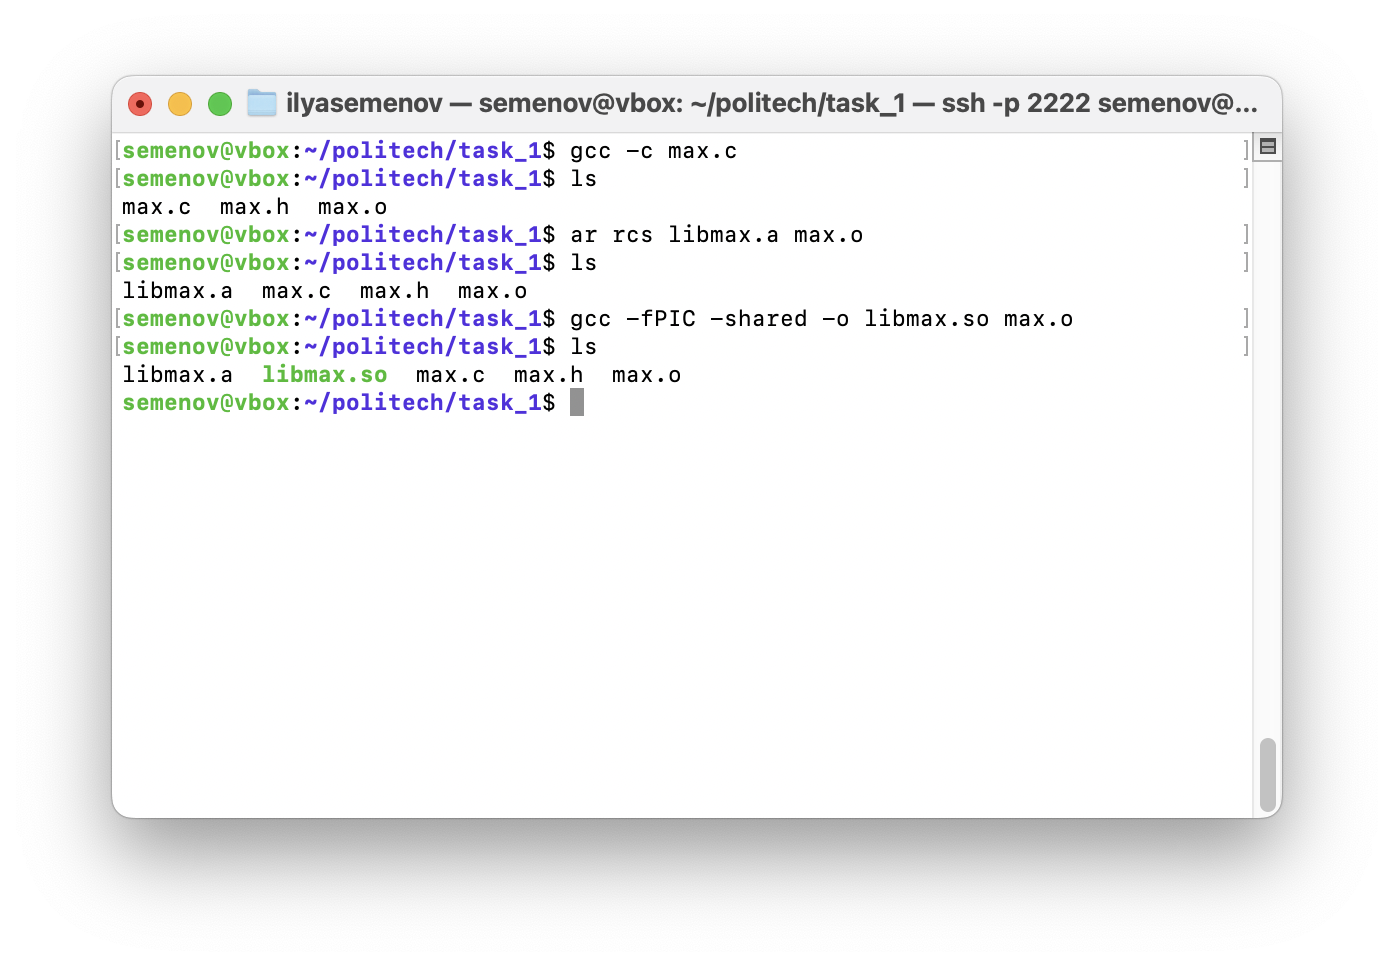
\includegraphics[width=0.85\textwidth]{img/Screenshot_2025-06-20_at_01.10.14.png}
\caption{Создание статической (\texttt{libmax.a}) и динамической (\texttt{libmax.so}) библиотек}
\end{figure}

\noindentВ результате сборки в папке находятся:
\begin{itemize}[noitemsep]
  \item \texttt{max.c}, \texttt{max.h} — исходные файлы;
  \item \texttt{max.o} — объектный файл;
  \item \texttt{libmax.a} — статическая библиотека;
  \item \texttt{libmax.so} — динамическая библиотека.
\end{itemize}

Таким образом, была успешно реализована и собрана библиотека поиска максимального элемента в массиве. Поддерживаются три типа данных и две стратегии реализации. Библиотека подготовлена как в виде статической, так и динамической и сопровождается блок-схемами, отражающими логику работы каждого варианта.

